% This file is part of JTS-MM (https://github.com/paulotto/jts-mm).
% SPDX-FileCopyrightText: 2026 Paul-Otto Müller
% SPDX-License-Identifier: CC-BY-4.0

\section{Spring design mathematics}\label{sec:springs}
All springs in this document are sized with the same few relations. The scripts evaluate them
(\texttt{s08\_springs.py}, inputs at the top and in \texttt{params.py}); the formulas are given here
so they can be checked and applied by hand. Verify every spring with a spring scale before use.

\subsection{Method: strain first, force second}\label{sec:method}
Every clamp in this document works the same way. The spring is printed or bent so that, mounted, it
is deflected by a \emph{preload} $\delta_0$ (over-closure or pre-spread). While the part is pushed
over the height of contour it is deflected further, to
\begin{equation}
\delta_\text{max} = \delta_0 + u ,
\end{equation}
where $u$ is the undercut that the jaw must pass (after block-out). Two requirements follow:
\begin{enumerate}
\item \textbf{Strain.} At $\delta_\text{max}$ the peak strain must stay below what the material
tolerates repeatedly: about \SI{1}{\percent} for PETG and rigid splint resins, \SI{1.5}{\percent}
for PA12, \SI{0.5}{\percent} for spring-hard stainless steel. For every bending spring the peak
strain depends only on geometry and deflection, \emph{not} on the width or on $E$. So the strain
limit fixes the \emph{shape} (length, radius, wall thickness).
\item \textbf{Force.} The preload $F_0=k\,\delta_0$ sets the retention. The stiffness $k$ is
proportional to the width of the spring, so once the shape is fixed, the width sets the force.
\end{enumerate}

\paragraph{Energy bound.} A spring of volume $V$ can store at most
$U=\eta\,V\,E\,\varepsilon^2/2$, where $\eta$ is a shape efficiency ($1/9$ for a straight
rectangular cantilever, $1/3$ for constant bending moment, $1$ for uniform compression). Since
$U = F_\text{max}\delta_\text{max}/2$,
\begin{equation}
V_\text{min} = \frac{F_\text{max}\,\delta_\text{max}}{\eta\,E\,\varepsilon_\text{allow}^2}.
\label{eq:energy}
\end{equation}
\Cref{tab:energy} evaluates this for \SI{3}{N} at \SI{0.5}{mm}. It explains in one line why dental
clasps are made of metal: a printed polymer spring needs roughly \SIrange{35}{70}{mm^3} of flexing
material per jaw, a steel wire about \SI{3}{mm^3}.

\begin{table}[H]\centering\small
\caption{Minimum spring volume for $F_\text{max}=\SI{3}{N}$ at $\delta_\text{max}=\SI{0.5}{mm}$, \cref{eq:energy}.}\label{tab:energy}
\begin{tabular}{l l S[table-format=1.2] S[table-format=2.1] S[table-format=2.0]}
\toprule
material & loading & {$\eta$} & {$\varepsilon_\text{allow}$ [\%]} & {$V_\text{min}$ [mm$^3$]}\\
\midrule
\inputrows{generated/energy_table.tex}
\bottomrule
\end{tabular}
\end{table}

\paragraph{Pull-off force.} A jaw pressing with normal force $N$ on a face inclined by $\alpha$ to
the path of insertion (from the undercut depth $u$ over the engaged height $z$,
$\tan\alpha=u/z$) must be pushed outward to remove the part. With friction coefficient $\mu$, a
force balance along and across the face gives
\begin{equation}
F_\text{pull-off} = N\,\frac{\tan\alpha+\mu}{1-\mu\tan\alpha}, \qquad N = k\,(\delta_0+u)
\label{eq:pulloff}
\end{equation}
per jaw. For small $\alpha$ this is simply $N(\alpha+\mu)$: retention comes from the undercut and
from friction in roughly equal parts.

% ---------------------------------------------------------------------------
\subsection{Printed C-loop (concept 2)}\label{sec:loop}
\paragraph{Model.} The loop is a curved cantilever: a circular arc of radius $R$ (to the wall
centre), wall thickness $t$ and width $w$, clamped at the root angle $a_1$ and carrying the rigid
jaw at $a_2$. Angles are measured in the section plane from the direction toward the tooth, so a
point of the arc sits at $(n,h) = (n_c+R\cos a,\; h_c+R\sin a)$. The tooth pushes on the jaw with a
force $P$ along $n$ at height $h_P$. The bending moment in the section at angle $a$ is
\begin{equation}
M(a) = P\,m(a),\qquad m(a) = e + R\sin a,\qquad e = h_c - h_P .
\end{equation}
Castigliano's theorem, bending energy only ($ds = R\,da$), gives the deflection of the jaw along $P$:
\begin{equation}
\delta = \frac{1}{EI}\int_{a_1}^{a_2} M\,\frac{\partial M}{\partial P}\,R\,da = \frac{P\,R\,J}{E\,I},
\qquad I=\frac{w\,t^3}{12},
\end{equation}
\begin{equation}
J = \int_{a_1}^{a_2} m^2\,da = e^2\Theta + 2eR\,(\cos a_1-\cos a_2) + R^2\left(\frac{\Theta}{2}-\frac{\sin 2a_2-\sin 2a_1}{4}\right),
\qquad \Theta = a_2-a_1 .
\label{eq:J}
\end{equation}
With $N$ identical loops in series (an S- or double loop), the compliances add:
\begin{equation}
k = \frac{E\,w\,t^3}{12\,N\,R\,J},\qquad
\varepsilon_\text{max} = K_W\,\frac{\delta_\text{max}\,t\,|m|_\text{max}}{2\,N\,R\,J}.
\label{eq:loop}
\end{equation}
$|m|_\text{max}$ is the largest lever along the arc, and $K_W$ is the Winkler correction for the
inner fibre of a thick curved beam, for a rectangular section
\begin{equation}
K_W = \frac{(r_n-r_i)\,/\,(t\,(R-r_n)\,r_i)}{6/t^2},\qquad r_i = R-\tfrac{t}{2},\quad r_n = \frac{t}{\ln\!\big((R+t/2)/r_i\big)} ,
\end{equation}
$K_W\approx1.10$ for $R/t=3.75$ and $\to1$ for slender loops.

\paragraph{The chosen geometry in closed form.} For a \SI{270}{\degree} loop ($a_1=-270^\circ$,
$a_2=0$) with the contact force passing through the loop centre ($e=0$), $J=3\pi R^2/4$ and
$|m|_\text{max}=R$, so
\begin{equation}
\boxed{\;k = \frac{E\,w\,t^3}{9\pi\,N\,R^3},\qquad \varepsilon_\text{max} = K_W\,\frac{2\,\delta_\text{max}\,t}{3\pi\,N\,R^2}\;}
\label{eq:loopbox}
\end{equation}
Putting the loop centre at the contact height ($e=0$) is deliberate: an offset $e$ increases $J$
only slightly but raises $|m|_\text{max}$ to $|e|+R$, so it costs strain for no gain in compliance.

\paragraph{Design procedure.}
\begin{enumerate}
\item Choose the material ($E$, $\varepsilon_\text{allow}$), the preload $\delta_0$ and the
block-out $u$; $\delta_\text{max}=\delta_0+u$.
\item Choose the wall $t$ from the printer: a multiple of the line width for FDM (\SI{0.8}{mm} =
two \SI{0.4}{mm} lines), anything from \SI{0.6}{mm} for SLA/DLP.
\item Radius from the strain limit:
$R \ge \sqrt{2K_W\,\delta_\text{max}\,t\,/\,(3\pi N\varepsilon_\text{allow})}$.
\item Width from the preload: $w = 9\pi N R^3 F_0/(E\,t^3\,\delta_0)$.
\item If $w$ does not fit next to the jaw (about \SI{7}{mm}), use $N=2$ or a larger $R$.
\end{enumerate}

\paragraph{Worked example (the geometry in the drawings).} PETG, $E=\SI{2}{GPa}$,
$\varepsilon_\text{allow}=\SI{1}{\percent}$; $\delta_0=\SI{0.2}{mm}$, $u=\SI{0.3}{mm}$, so
$\delta_\text{max}=\SI{0.5}{mm}$; $t=\SI{0.8}{mm}$, $N=1$, $K_W=1.1$:
\[
R \ge \sqrt{\frac{2\cdot1.1\cdot0.5\cdot0.8}{3\pi\cdot0.01}} = \SI{3.06}{mm}\ \Rightarrow\ R=\SI{3.0}{mm}
\quad(\varepsilon_\text{max}=\SI{1.03}{\percent}),
\]
\[
w = \frac{9\pi\cdot27\cdot1.5}{2000\cdot0.512\cdot0.2} = \SI{5.6}{mm}\ \Rightarrow\ w=\SI{5.5}{mm},
\quad k=\SI{7.4}{N/mm},\ F_0=\SI{1.5}{N},\ F_\text{max}=\SI{3.7}{N}.
\]

\begin{figure}[H]\centering
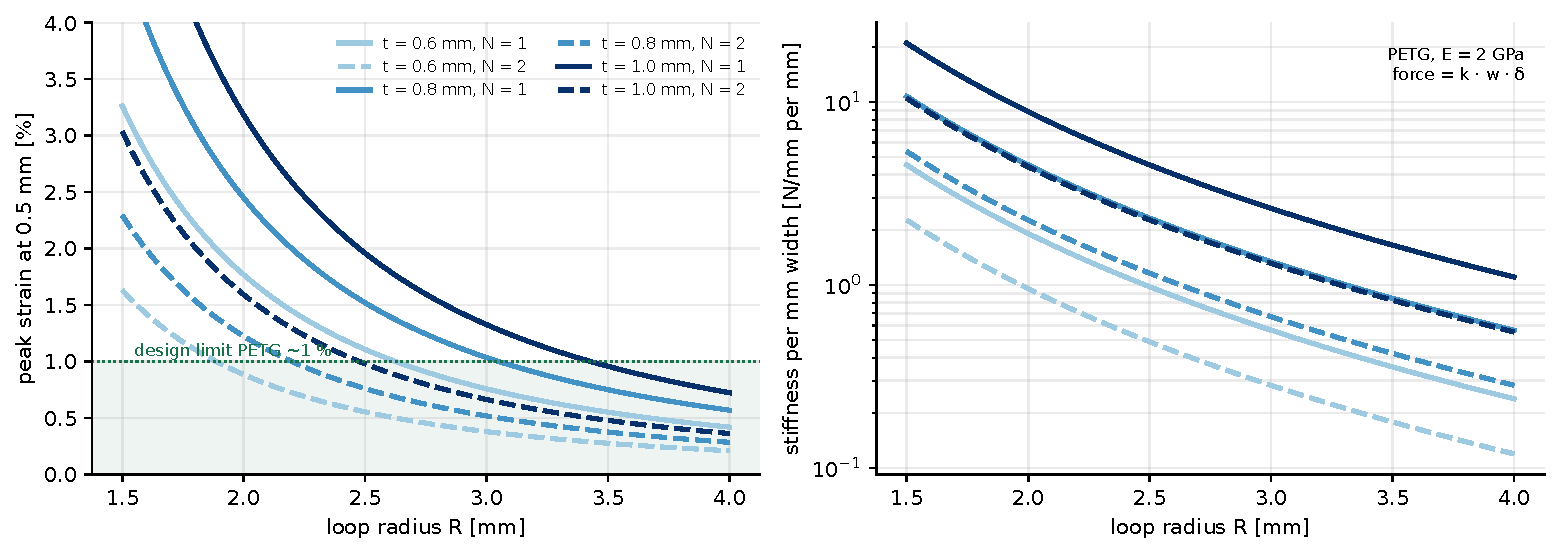
\includegraphics[width=\textwidth]{springs_loop}
\caption{C-loop design chart ($e=0$, \SI{270}{\degree}, PETG). Left: peak strain at
$\delta_\text{max}=\SI{0.5}{mm}$ picks $R$ for a given $t$ and number of loops $N$ (solid $N=1$,
dashed $N=2$); it does not depend on $w$ or $E$. Right: stiffness per millimetre of width; multiply
by $w$ and $\delta_0$ for the preload.}
\label{fig:loopchart}
\end{figure}

\begin{table}[H]\centering\small
\caption{C-loop options, PETG, $\delta_0=\SI{0.2}{mm}$, $\delta_\text{max}=\SI{0.5}{mm}$, $e=0$.
Red: above the strain limit. Arrow: the geometry in the drawings. The first row is the loop of an
earlier design: about three times stiffer than first estimated, and overstrained.}\label{tab:loop}
\begin{tabular}{c S[table-format=1.1] S[table-format=1.1] S[table-format=1.1] S[table-format=2.1] S[table-format=2.1] S[table-format=1.1] S[table-format=1.2] c}
\toprule
{$N$} & {$R$ [mm]} & {$t$ [mm]} & {$w$ [mm]} & {$J$ [mm$^2$]} & {$k$ [N/mm]} & {$F_0$ [N]} & {$\varepsilon_\text{max}$ [\%]} & \\
\midrule
\inputrows{generated/loop_table.tex}
\bottomrule
\end{tabular}
\end{table}

\paragraph{Printing the loop.}
\begin{itemize}
\item Print the loop module flat, loop plane in the build plane, so bending stays within layers.
\item Wall = whole extrusion lines; \SI{100}{\percent} infill is automatic at two lines. No
ironing or top skin across the loop.
\item Fillet the root (radius $\ge\SI{0.5}{mm}$): the root carries the largest moment.
\item Print it over-closed by $\delta_0$ (the jaw sits $\delta_0$ closer to the tooth than on the
model). Measure $F$ at $\delta_0$ and $\delta_\text{max}$; if needed change $w$, keep $t$ and $R$.
\item Polymers relax: after \SI{30}{min} at \SI{37}{\celsius} the force can be noticeably lower.
Size for the relaxed value, or accept re-printing.
\end{itemize}

% ---------------------------------------------------------------------------
\subsection{Straight clasp arm (alternative for concepts 1 and 2)}
A straight arm of length $L$ along the tooth, height $b$ and thickness $t$ (normal to the tooth),
clamped at the embrasure end:
\begin{equation}
k = \frac{E\,b\,t^3}{4L^3},\qquad \varepsilon_\text{max} = \frac{3\,t\,\delta_\text{max}}{2L^2}
\quad\Rightarrow\quad L \ge \sqrt{\frac{3\,t\,\delta_\text{max}}{2\,\varepsilon_\text{allow}}}.
\end{equation}
It lies flat against the lingual face and needs no tongue space, but a polymer arm that fits along
one molar gives little force (\cref{tab:arm}).
\begin{table}[H]\centering\small
\caption{Straight PETG clasp arm, $\delta_0=\SI{0.2}{mm}$, $\delta_\text{max}=\SI{0.5}{mm}$.}\label{tab:arm}
\begin{tabular}{S[table-format=2.0] S[table-format=1.0] S[table-format=1.1] S[table-format=1.1] S[table-format=1.1] S[table-format=1.2]}
\toprule
{$L$ [mm]} & {$b$ [mm]} & {$t$ [mm]} & {$k$ [N/mm]} & {$F_0$ [N]} & {$\varepsilon_\text{max}$ [\%]}\\
\midrule
\inputrows{generated/arm_table.tex}
\bottomrule
\end{tabular}
\end{table}

% ---------------------------------------------------------------------------
\subsection{Stainless arch wire (concept 4)}
Each leg of the arch is a cantilever from the rigid yoke to the molar pad, length
$L=\SI{17.6}{mm}$ (measured on the concept geometry), $E=\SI{185}{GPa}$:
\begin{equation}
k = \frac{3EI}{L^3},\quad I=\frac{\pi d^4}{64},\qquad F_0 = k\,\delta_0,\qquad
\sigma_\text{max} = \frac{3E\,(\delta_0+u)\,d/2}{L^2},
\end{equation}
and the pull-off force from \cref{eq:pulloff} with $z=\SI{3}{mm}$, $\mu=0.1$.

\begin{figure}[H]
\centering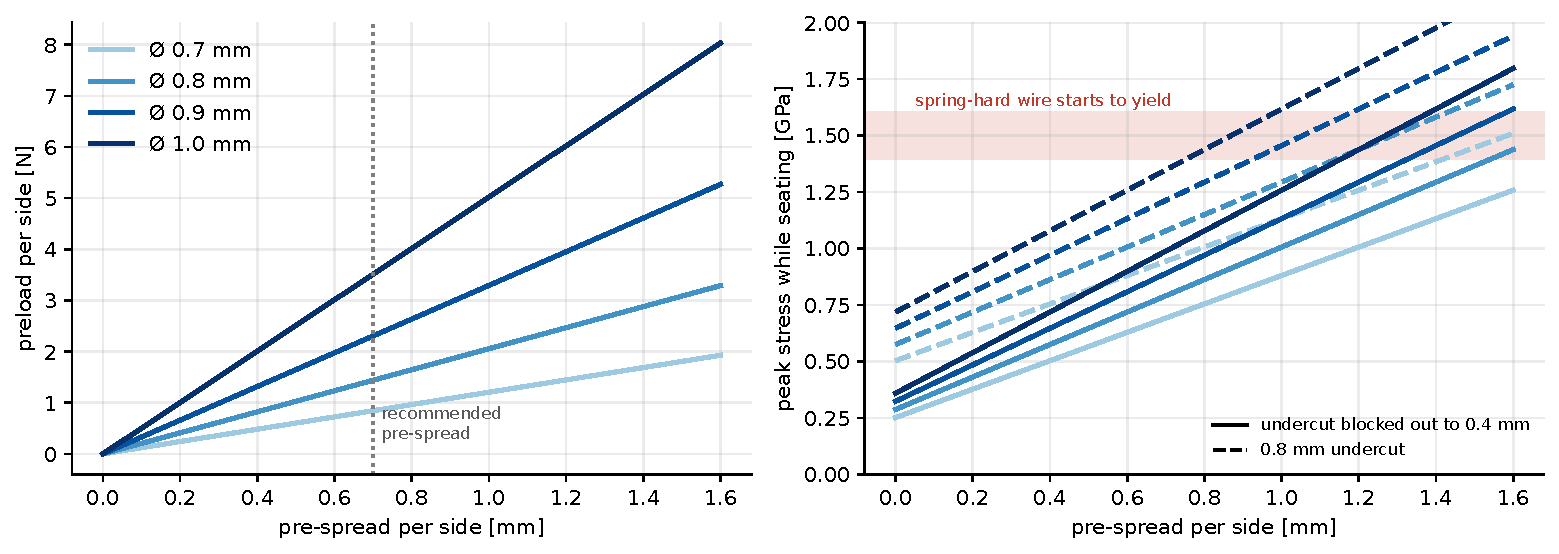
\includegraphics[width=\textwidth]{springs_wire}
\caption{Preload (left) and peak stress while seating (right) versus pre-spread. Red band: proof
stress of spring-hard wire (about \SIrange{1.4}{1.6}{GPa}).}
\label{fig:springs}
\end{figure}

\begin{table}[H]\centering\small
\caption{Arch wire, per side. Red: at or above the yield band.}\label{tab:wire}
\begin{tabular}{S[table-format=1.1] S[table-format=1.1] S[table-format=1.1] S[table-format=1.1] S[table-format=1.1] S[table-format=1.2] S[table-format=1.1]}
\toprule
{$d$ [mm]} & {$\delta_0$ [mm]} & {$u$ [mm]} & {$k$ [N/mm]} & {$F_0$ [N]} & {$\sigma_\text{max}$ [GPa]} & {$F_\text{pull-off}$ [N]}\\
\midrule
\inputrows{generated/wire_table.tex}
\bottomrule
\end{tabular}
\end{table}

\begin{keybox}
\textbf{The limit is stress, not force.} At fixed deflection the peak stress grows linearly with the
wire diameter, so a thicker wire yields \emph{sooner}. Use \textbf{\SI{0.9}{mm}, \SI{0.7}{mm}
pre-spread, undercut blocked out to \SI{0.4}{mm}}: \SI{\approx2.3}{N} preload, \SI{\approx0.9}{GPa}
peak. For the Adams clasps of concept~3, \SI{0.7}{mm} is the established size on permanent molars.
\end{keybox}

% ---------------------------------------------------------------------------
\subsection{TPU liner (concept 5)}
A liner of thickness $t_l$ squeezed by the interference $\delta$ over the contact area $A$:
\begin{equation}
F = E_c\,\varphi\,A\,\frac{\delta}{t_l},\qquad E_c \approx E\,(1+2\kappa S^2),\qquad S = \frac{A}{p\,t_l},
\end{equation}
with $\varphi$ the solid fraction of the liner, $p$ the perimeter of the loaded area, and the shape
factor $S$ stiffening a solid pad that cannot bulge sideways ($\kappa\approx0.6$--$0.9$). For the
contact band \SI{7}{mm}$\times$\SI{1.5}{mm} and $t_l=\SI{1.6}{mm}$ a solid pad has $E_c\approx1.8E$;
free-standing ribs have $E_c\approx E$. Tensile moduli \SI{12}{MPa} (85A) and \SI{26}{MPa} (95A).
\begin{table}[H]\centering\small
\caption{TPU liner force in N for a given interference.}\label{tab:tpu}
\begin{tabular}{l l S[table-format=2.0] S[table-format=2.0] S[table-format=2.0]}
\toprule
grade & liner & {\SI{0.1}{mm}} & {\SI{0.2}{mm}} & {\SI{0.3}{mm}}\\
\midrule
\inputrows{generated/tpu_table.tex}
\bottomrule
\end{tabular}
\end{table}
A ribbed 85A or 95A liner with \SIrange{0.1}{0.2}{mm} interference lands in the useful
\SIrange{3}{12}{N} range and tolerates print error; a solid liner is far too stiff and makes the
preload depend on hundredths of a millimetre. TPU moduli vary between brands: treat these numbers
as orders of magnitude.
